% !TEX root = ../../UPDATED_main.tex
\subsection*{SatuTe localizes alignment-specific losses in Tree-of-Life data}

We revisited two alignments used for deep Tree-of-Life inference \cite{hug2016}: 2,596 amino-acid sites from 16 ribosomal proteins across 3,083 taxa, supporting a two-domain (2D) tree; and 1,947 16S rRNA sites across 1,871 taxa, supporting a three-domain (3D) tree. Branch lengths were re-estimated under LG+G4 and GTR+G4, respectively. We tested the internal branch leading to Eukaryota and an external yeast branch (Supplementary Fig. S2).

In the protein 2D tree, original SatuTe classified all 6,163 branches as informative in each of the four rate categories. In the fastest rRNA category (rate 2.73), it classified 107 of 3,739 branches as saturated; 13 were internal, including the Eukaryota branch.

Sliding windows localized this contrast (Fig.~\ref{fig-biological-windows}). Original SatuTe classified 822 of 1,912 rRNA windows (43.0\%) as saturated for the Eukaryota branch, compared with 138 of 2,561 protein windows (5.4\%). Protein losses were short and often coincided with boundaries in the concatenation. rRNA losses were enriched in hypervariable regions V1--V9 \cite{baker2004}; conserved regions C1 and C4--C9 retained signal, whereas C2 and C3 were nearly saturated. Gappy intervals at positions 240--301 and 789--956 contributed little information.

The weighted sensitivity analysis reduced, but did not erase, this pattern. Native dominant and weighted analyses classified 895 and 699 rRNA windows as saturated for Eukaryota, and 83 and 29 for yeast, respectively. In the protein alignment, original dominant and native weighted analyses classified 138 and 5 windows as saturated for Eukaryota, and 54 and 8 for yeast. Because these cross-implementation comparisons also differ in input handling, the paired simulations provide the controlled estimate of the formula effect.

\begin{figure}[p]
  \centering
  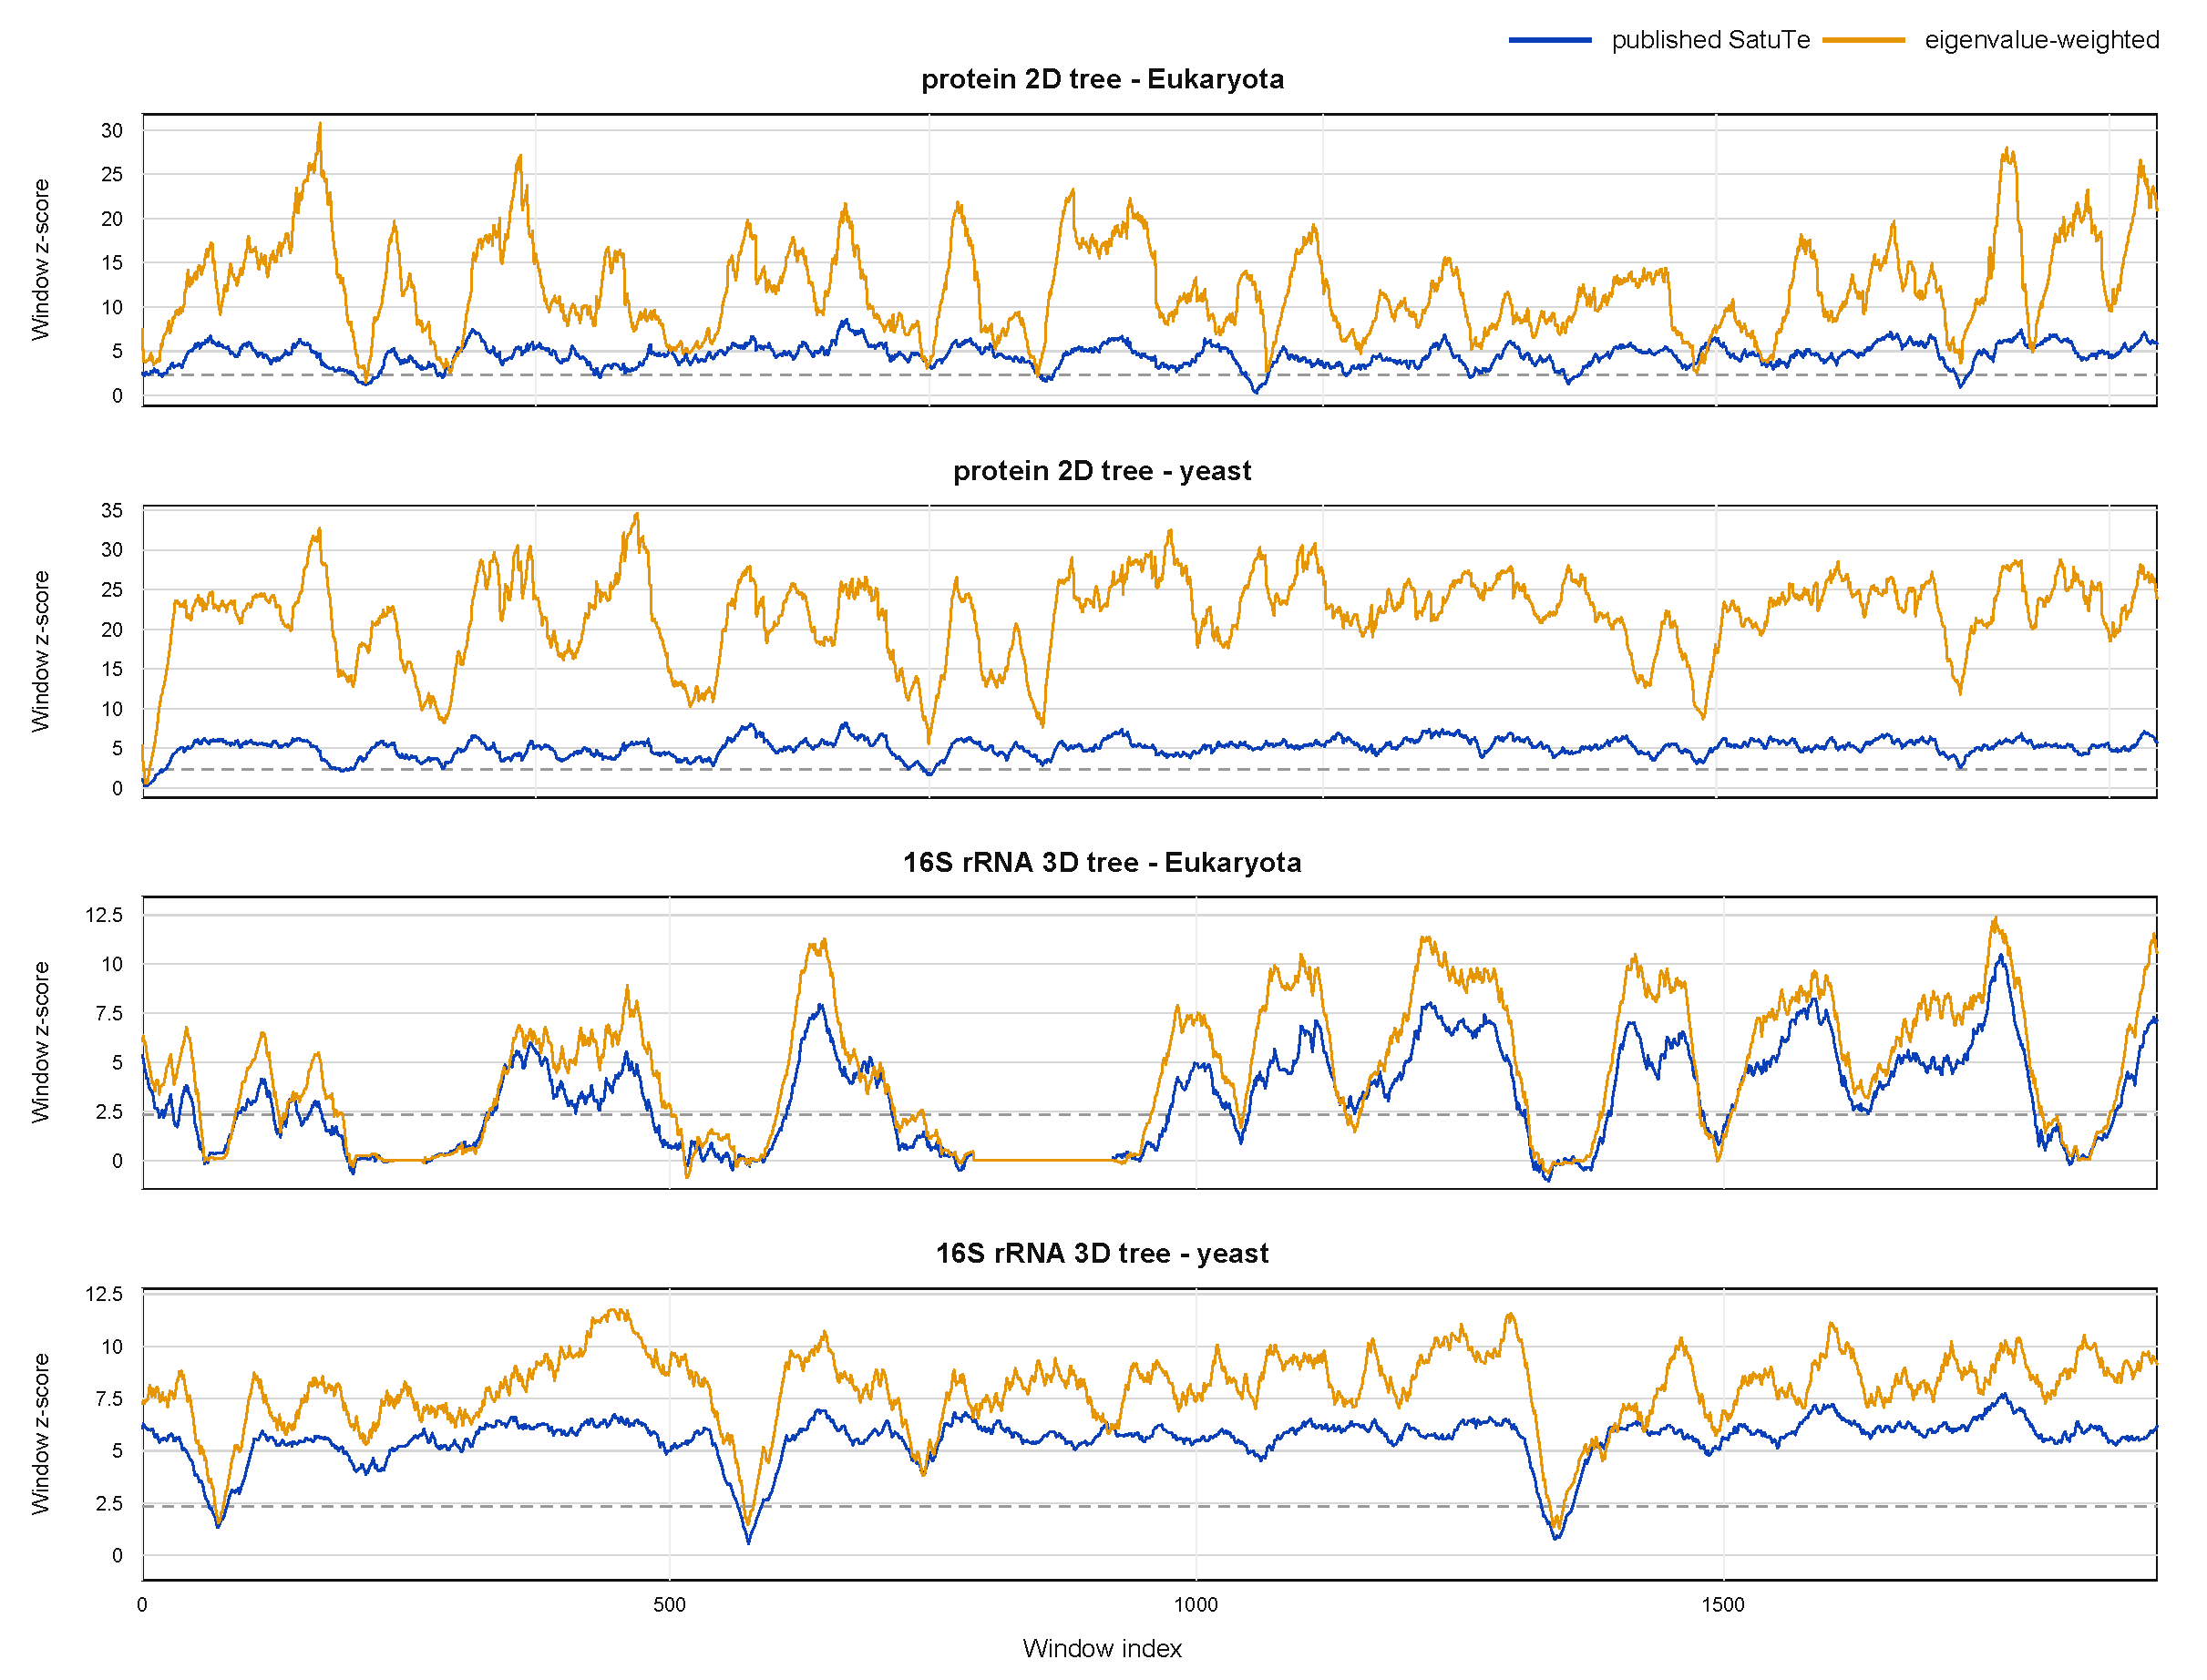
\includegraphics[width=0.66\textwidth]{figures/published_vs_eigenvalue_weighted_curves.pdf}
  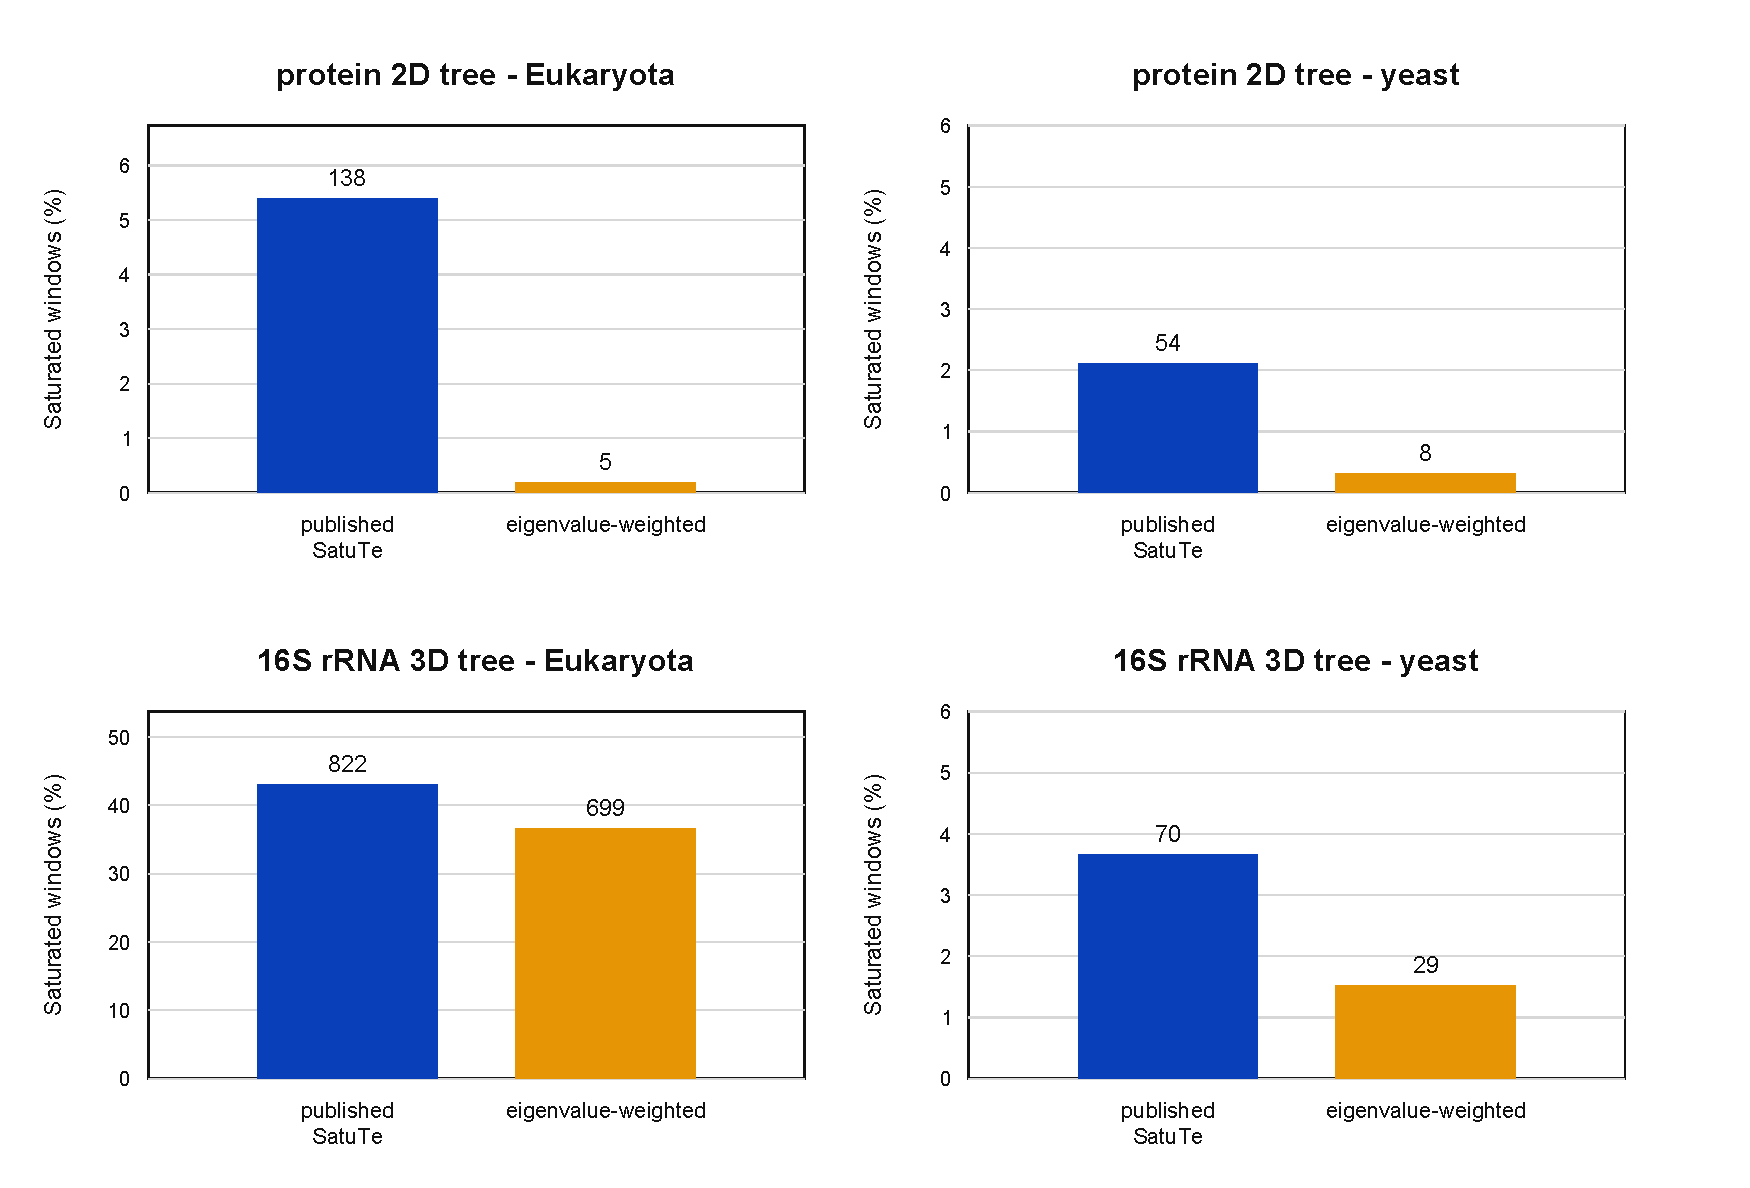
\includegraphics[width=0.66\textwidth]{figures/published_vs_eigenvalue_weighted_saturated_windows.pdf}
  \caption{\textbf{Branch-specific signal across Tree-of-Life alignments.} \textbf{a,} Thirty-six-site window \(Z\)-scores for Eukaryota and yeast branches in protein 2D and rRNA 3D trees; the dashed line marks the decision threshold. \textbf{b,} Fractions and counts of saturated windows. Weighting changes threshold crossings most strongly for the rRNA Eukaryota branch but preserves the protein--rRNA contrast established by original SatuTe.}
  \makeatletter\cref@old@label{fig-biological-windows}\makeatother
\end{figure}

All 16 ribosomal proteins produced significant scores under both 2D and rearranged 3D placements of Eukaryota; L15, L22, and S10 favored the rearranged placement. Six of nine rRNA regions had larger scores under the 3D placement. The two distributions of score differences did not differ significantly (Kolmogorov--Smirnov \(p=0.072\)). These results localize signal for candidate placements rather than select a true topology (Supplementary Tables S4 and S5).

\subsection*{SatuTe exposes codon-position-specific losses in HCV}

An independent hepatitis C virus (HCV) reference panel provided a coding-genome example spanning seven recognized genotypes \cite{smith2014}. Every complete gene and codon-position partition retained signal, but 36-site \(Z\)-score curves revealed localized losses (Fig.~\ref{fig-hcv-windows}). Across genotype 1, 2, and 3 branches, original SatuTe classified 1/507, 4/507, and 5/507 position-1+2 windows as saturated, compared with 11/252, 34/252, and 33/252 third-position windows. Eigenvalue weighting reduced the corresponding third-position counts to 6, 24, and 27 (Supplementary Table S6).

A gene-level screen would therefore retain every locus, whereas SatuTe profiles reveal signal loss associated with third positions and specific intervals. These profiles can motivate partition-specific model checks or selective masking without requiring wholesale removal of otherwise informative genes.

\begin{figure}[p]
  \centering
  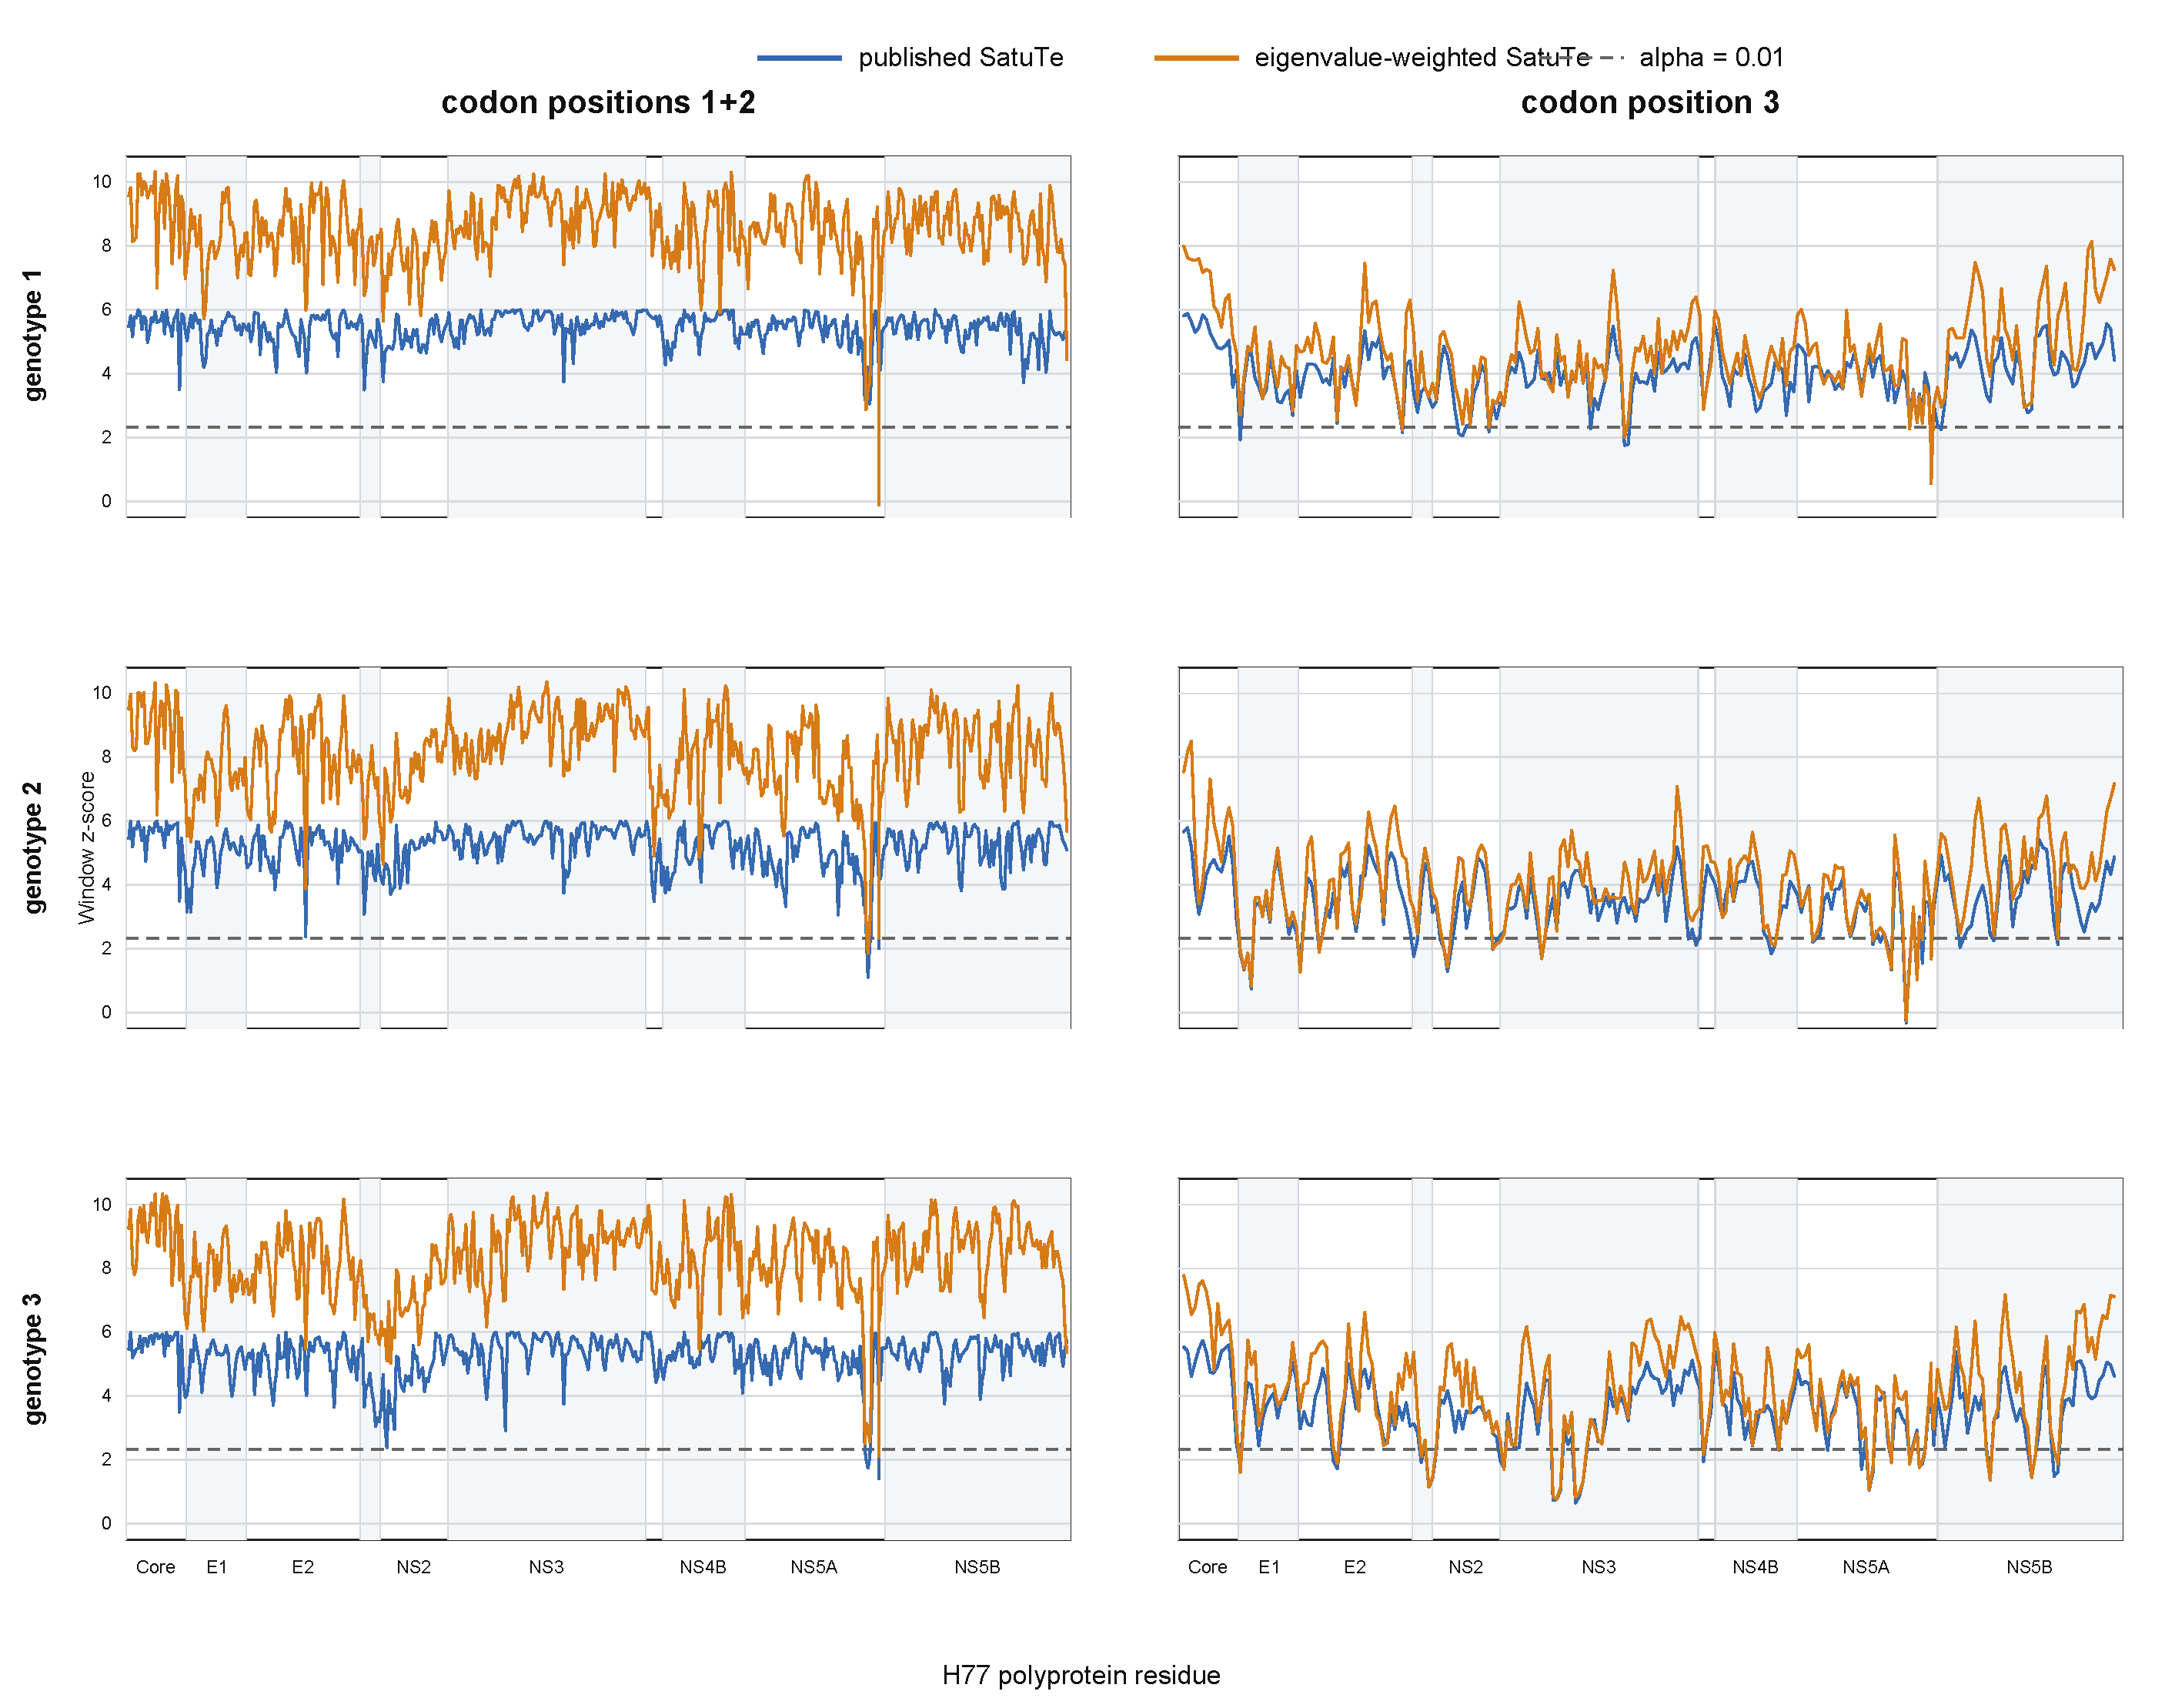
\includegraphics[width=0.92\textwidth]{figures/hcv_codon_position_window_curves.pdf}
  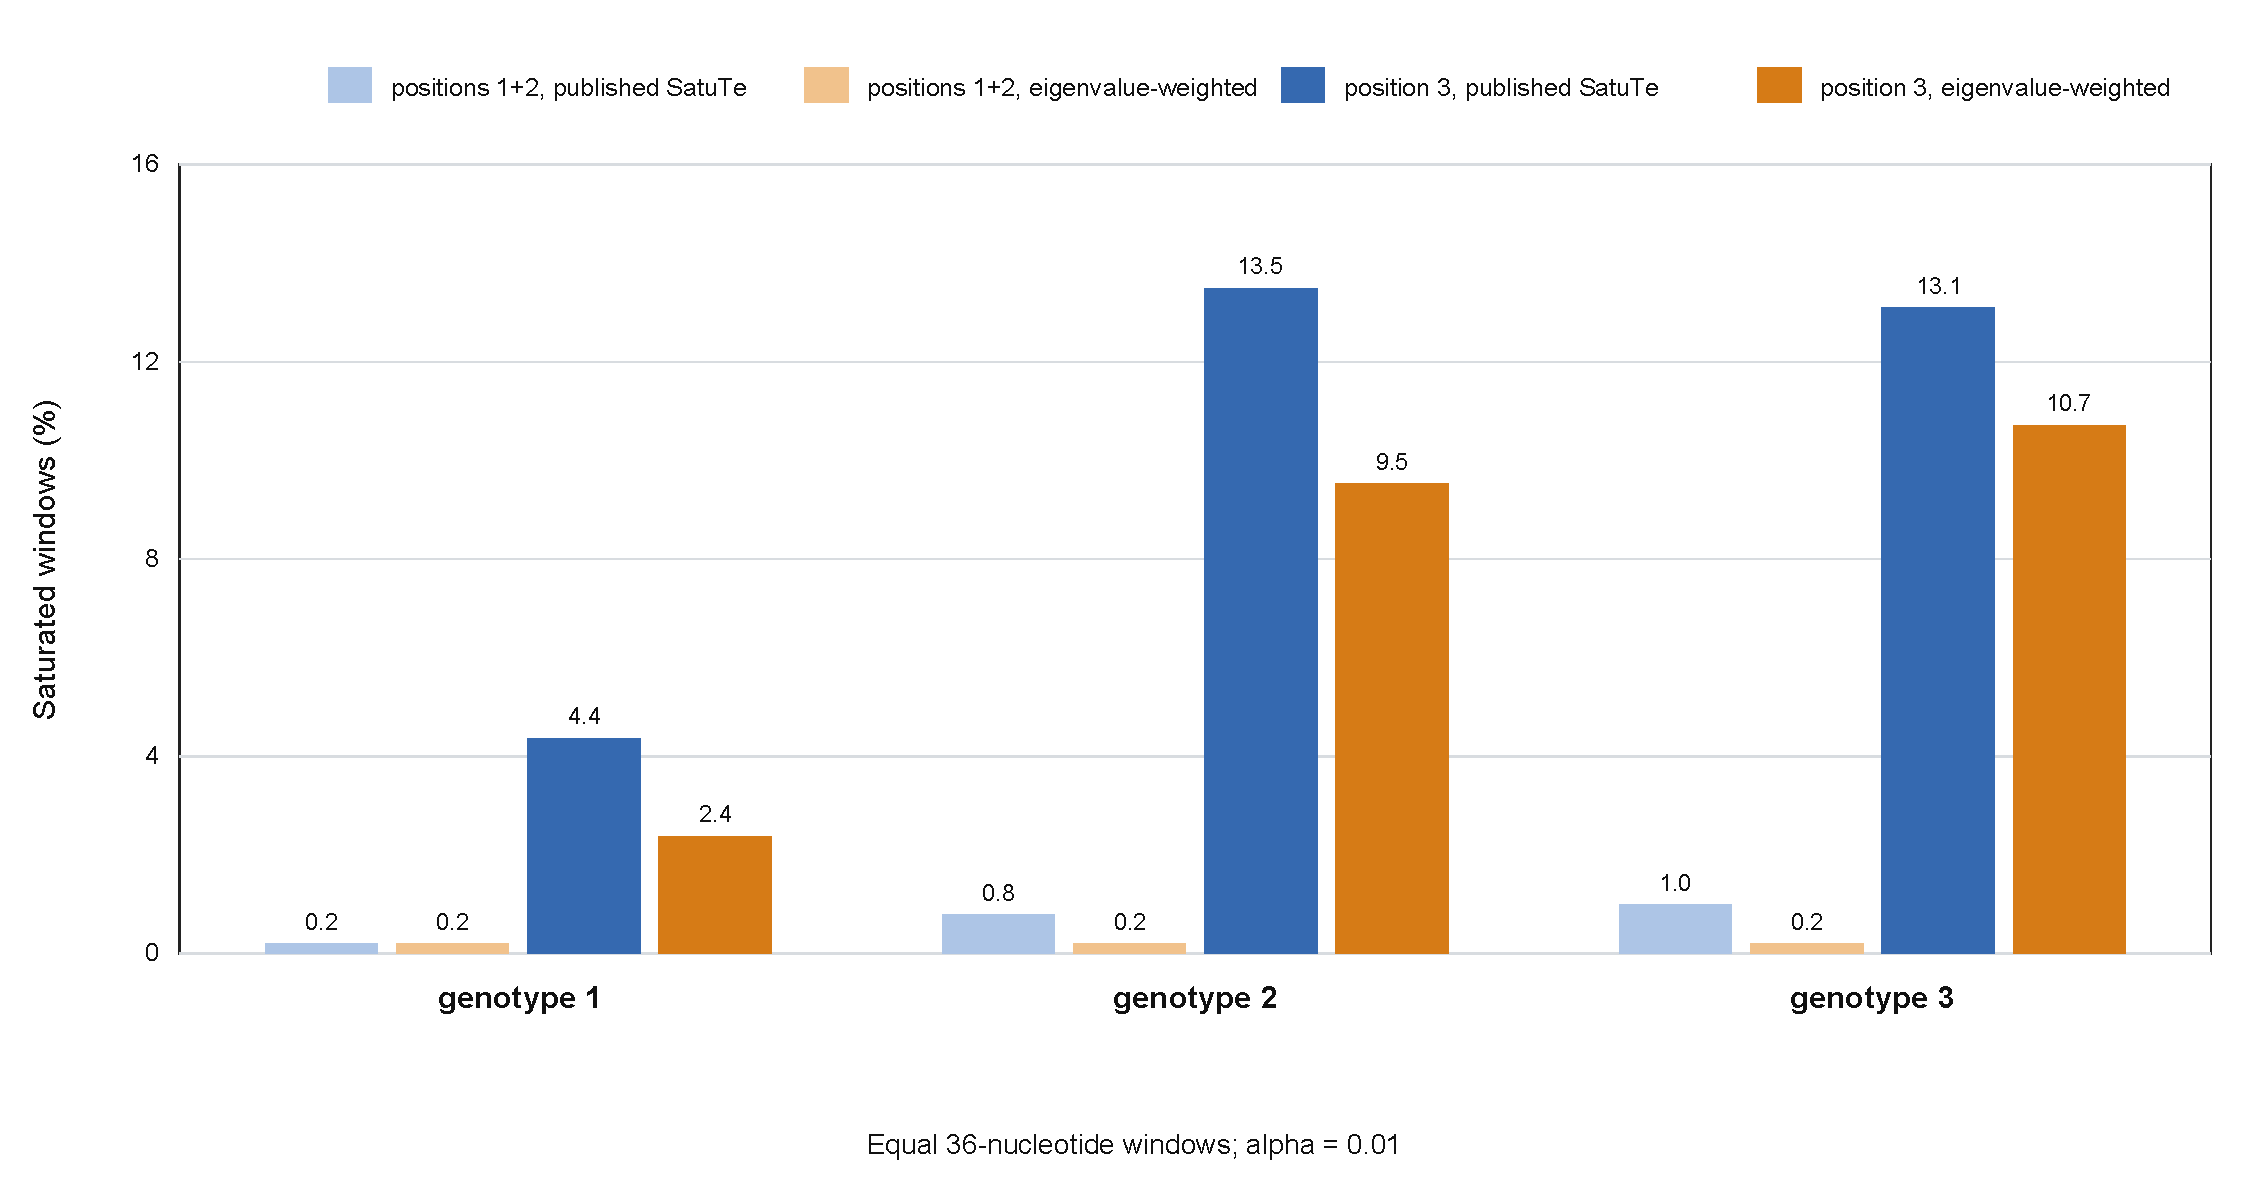
\includegraphics[width=0.80\textwidth]{figures/hcv_codon_position_saturated_windows.pdf}
  \caption{\textbf{Codon-position localization in an HCV reference panel.} \textbf{a,} Original and eigenvalue-weighted SatuTe \(Z\)-scores along the H77 polyprotein coordinate for fixed-topology 36-site windows. The dashed line marks the descriptive \(\alpha=0.01\) threshold. \textbf{b,} Fractions of saturated windows. Losses concentrate in the synonymous-enriched third-position partition; weighting reduces, but does not remove, the pattern concealed by whole-gene tests.}
  \makeatletter\cref@old@label{fig-hcv-windows}\makeatother
\end{figure}
